\documentclass[conference]{IEEEtran}
\IEEEoverridecommandlockouts%

% Packages
\usepackage{cite}
\usepackage{amsmath,amsfonts}
\usepackage{algorithm}
\usepackage{algpseudocode}
\usepackage{graphicx}
\usepackage{textcomp}
\usepackage{xcolor}
\usepackage{booktabs}
\usepackage{adjustbox}
\usepackage{listings}
\usepackage{bm}
\usepackage{hyperref}

\usepackage{pgfplots}
\pgfplotsset{compat=newest}
\usepackage{siunitx}

\usepackage{verbatim}
\usepackage{multirow}

\graphicspath{{./img/}}

\def\BibTeX{{\rm B\kern-.05em{\sc i\kern-.025em b}\kern-.08em
    T\kern-.1667em\lower.7ex\hbox{E}\kern-.125emX}}

\begin{document}

\title{Deliverable report \\
\footnotesize \textit{``Alessio Blascovich'': Mat: 257561, \texttt{alessio.blascovich@studenti.unitn.it}, GitRepo: \texttt{https://github.com/elblasco/GPU-Computing-2025-257561}}}

\maketitle

\begin{abstract}
%[max 200 words]\\
The sparse matrix-dense vector multiplication (SpMV) is an algebraic operation in which a sparse matrix is multiplied by a dense vector. SpMV is widely used in real-world applications such as scientific and engineering computing, data mining, and graph analysis.

This deliverable discusses the implementation and the performance analysis of a series of SpMV algorithms for COO matrices. These algorithms are implemented for a single-core CPU and a \emph{CUDA} capable GPU. Regarding the GPU implementations, no threads/warp level synchronisation has been used, only atomic operations to keep the resulting vector consistent.
\end{abstract}

\begin{IEEEkeywords}
Sparse Matrix, SpMV, \emph{CUDA}, Parallelization, Storage Format
\end{IEEEkeywords}

\section{Introduction}
SpMV is considered a fundamental algebraic operation in many scientific fields such as computational fluid dynamics, optimisation and graph algorithms.

The main challenges in implementing an efficient SpMV algorithm differ in CPU and GPU, and are strictly bound to the type of matrix representation used (COO, CSR, ELL,\dots). For the purpose of this deliverable only COO representation is taken into account.

From the CPU point of view, the main issue is to maximise the cache hits throughout the execution, data consistency is not a problem since only single core CPUs were used.

On the GPU side the problem of maximising cache hits remains, and on top of that, race conditions are added. Since in COO format the length of a row is not specified, multiple threads could be reading different portions of the same row and therefore, writing on the same output memory area.

\section{Problem Statement}
The SpMV operation is formally defined in Equation~\ref{eq:1}, where \(\bm{A}\) is a \(n\times m\) sparse matrix, \(\bm{x}\) a \(m\times 1\) dense vector and \(\bm{y}\) another \(n\times 1\) dense vector.

\begin{equation}\label{eq:1}
\bm{y} = \bm{Ax}
\end{equation}

\subsection{Storage Format}
The coordinate (COO) format is a representation of sparse matrix. COO uses 3 different arrays to store al the necessary information. One array dedicated to store all the non-zero values, while the other 2 contain the corresponding row and column indices. For the sake of simplicity, all the input matrices are assumed to be sorted in row-major order, this is done by transposing all the input matrices which were sorted in column-major order.

\subsection{Parallelization}
2 different kernels have been used for the \emph{CUDA} capable GPU, although in both of them the workload is divided equally among all the threads used. The main difference is the pattern used to access the global memory from a thread. In the first approach each thread jumps of stride equivalent to the number of threads used, while in the second approach a thread access to a continuos area of memory long as the total number of non-zero element in the matrix divided by the number of threads used.

\section{State of the Art}
%Describe the available library solutions for the SpMV problem, including references and citations \cite{asimov1950irobot, svevo1923coscienza, pirandello1926uno}.
Starting from the implementations presented in this deliverable, performances could be drastically enhanced. Fukaya et al.~\cite{fukaya2021}, despite focussing on the HDC storage format, improved the SpMV CPU based by exploiting diagonalization patterns, SIMD instructions and \emph{OpenMP} directives. On the GPU side Chu et al.~\cite{chu2023} used the CSR format and a more sophisticated load balancing to improve the performances. NVIDIA itself made available a set of libraries to manage and use COO formatted matrices, namely \textit{cuSPARSE}.
\section{Methodology and Contributions}\label{sec:methodology}

%Describe the methodology used during the analysis, the compared algorithms and the expected outcomes. Use pseudo-codes like Algorithm \ref{alg:COOaggr} to describe your own implemented kernels.

The tests has been carried out performing multiple rounds of caches warm up and then executing the various algorithm after. The data have been collected throughout the execution since only for the first warm up cycle there were substantially data variations.

\subsection{CPU implementation}

% \noindent Include at least the following implementations:
% \begin{itemize}
%     \item Naive CPU implementation
%     \item Optimised CPU implementation based on cache behaviour
%     \item GPU naive implementation
% \end{itemize}

% \noindent For the analysis include
% \begin{itemize}
%     \item Valgrind and runtime comparison between the CPU implementations 
%     \item Runtime CPU vs GPU comparison looping over different matrix dimensions
% \end{itemize}

The CPU simply loop through all the elements and performs the operations required for the matrix multiplication element-wise. The CPU Algorithm~\ref{alg:cpu} maximise the cache hit since it reads, sequentially, elements that are stored in a contiguous memory area, this holds for \texttt{res[row[i]]} and \texttt{val[i]}.

\begin{algorithm}[h]
\caption{SpMV algorithm on CPU}
\algorithmicrequire~The input vectors \(val\), \(row\) and \(col\) of size \(nnz\), array \(arr\) of size \(columns\) and an array \(res\) of size \(rows\).
\begin{algorithmic}[1]
\Procedure{Function}{\(row\), \(col\), \(val\), \(arr\), \(res\), \dots}
  \While{\(i\) in \(\{0\dots nnz\}\)}
    \State\(res[row[i]] = res[row[i]] + (val[i] \cdot arr[col[i]])\)
    \State\(i = i + 1\)
  \EndWhile%
\EndProcedure%
\end{algorithmic}
\label{alg:cpu}
\end{algorithm}

In particular instance I had to use my personal computer since the cluster version of \emph{valgrind} has some trouble with the cache profile tool. Due to hardware limitation I performed the cache profiling using smaller matrices. To have clearer I did not perform any warm-up cycle sine I want to measure the effectiveness of my algorithm on ``pseudo-empty'' caches.

\begin{table}[h]
  \centering
    \begin{tabular}{c|c c}
      \toprule
      Matrix & D1 read & D1 write\\
      \midrule
      \texttt{lp\_nug05} & 1.5\% & .5\%\\
      \texttt{rdb250l} & .8\% & .3\%\\
      \texttt{fpga\_dcop\_15} & .3\% & .2\%\\
      \bottomrule
    \end{tabular}
  \vspace{.5em}
  
  \caption{L1 cache misses}
  \label{tab:L1miss}
\end{table}

\begin{table}[h]
  \centering
    \begin{tabular}{c|c c}
      \toprule
      Matrix & LLd read & LLd write\\
      \midrule
      \texttt{lp\_nug05} & .7\% & .3\%\\
      \texttt{rdb250l} & .4\% & .2\%\\
      \texttt{fpga\_dcop\_15} & .1\% & .1\%\\
      \bottomrule
    \end{tabular}
  \vspace{.5em}
  
  \caption{L2 and L3 cache misses}
  \label{tab:L2L3miss}
\end{table}

\subsection{GPU}

For the GPU implementation I have created two kernel, they differ on the access pattern used for the memory. In Algorithm~\ref{alg:striding} every thread jumps to the next element which has index \emph{current index + \texttt{numThreads}}. In Algorithm~\ref{alg:contiguous} each thread accesses \texttt{portion} elements which are stored in a contiguous area of memory.

\begin{algorithm}[h]
\caption{SpMV algorithm with striding}
\algorithmicrequire~The input vectors \(val\), \(row\) and \(col\) of size \(nnz\), array \(arr\) of size \(columns\), an array \(res\) of size \(rows\) and a number \(portion\).
\begin{algorithmic}[1]
\Procedure{Function}{\(row\), \(col\), \(val\), \(arr\), \(res\), \dots}
  \State\(start\gets threadId\)
  \State\(end\gets(portion\cdot numThreads) + start\)
  \While{\(i\) in \(\{start\dots\min\{end, nnz\}\}\)}
    \State\(atomicAdd(\&res[row[i]], val[i] \cdot arr[col[i]])\)
    \State\(i = i + numThreads\)
  \EndWhile%
\EndProcedure%
\end{algorithmic}
\label{alg:striding}
\end{algorithm}

\begin{algorithm}[h]
\caption{SpMV algorithm with contiguous chunk}
\algorithmicrequire~The input vectors \(val\), \(row\) and \(col\) of size \(nnz\), array \(arr\) of size \(columns\), an array \(res\) of size \(rows\) and a number \(portion\).
\begin{algorithmic}[1]
\Procedure{Function}{\(row\), \(col\), \(val\), \(arr\), \(res\), \dots}
  \State\(start\gets portio\cdot threadId\)
  \State\(end\gets portion + start\)
  \While{\(i\) in \(\{start\dots\min\{end, nnz\}\}\)}
    \State\(atomicAdd(\&res[row[i]], val[i] \cdot arr[col[i]])\)
    \State\(i = i + 1\)
  \EndWhile%
\EndProcedure%
\end{algorithmic}
\label{alg:contiguous}
\end{algorithm}

From the theory Algorithm~\ref{alg:striding} should have been faster. This follows from the fact that every thread within the same SM (Streaming Multiprocessor) accesses elements that are spacially adjacent in the memory. Contrary, Algorithm~\ref{alg:contiguous} has an higher rate of cache miss since, threads in the same SM may need to access elements far away from each other. Since the cache optimisation is so important for these algorithm and they had to do so few floating point operations I expected for them to be memory bounded.

\section{System Description and Experimental Set-up}

%Use this section to describe system, dataset and experimental set-up.

\subsection{System Description}

%Describe the used system and the software environment (CUDA version, GCC version, \dots). Decide which information are valuable to group into a table like Table \ref{tab:system_description} and which are more valuable to be described in the text.

Table~\ref{tab:systems_softwares} shows the various software used in the deliverable, excluded the building tools. It is worth mentioning again that, for \emph{valgrind}, I had to do a rollback on my pc since the last version (same of the cluster) has some problem with the tool \emph{cachegrind}. 

\begin{table}[ht]
    \centering
    \begin{tabular}{lllr}
    \toprule
    \textbf{System} &  \textbf{GCC} & \textbf{Valgrind} & \textbf{CUDA}\\
    \midrule
    Cluster &  11.5.0 & 3.23.0 & 12.5.0\\
    PC &  15.1.1 & 3.20.0 & 12.8.1\\
    \bottomrule
    \end{tabular}
    \vspace{.5em}
    
    \caption{Systems softwares}
    \label{tab:systems_softwares}
\end{table}

\begin{table}[ht]
    \centering
    \begin{adjustbox}{width=\columnwidth}
    \begin{tabular}{lllrl}
    \toprule
    \textbf{System} &  \textbf{Processor} & \textbf{Cores per Socket} & \textbf{RAM} & \textbf{Accelerator} \\
    \midrule
    Cluster &  Intel(R) Xeon(R) Silver 4214 & 48 at 2.2 GHz & 400 GB & NVidia A30\\
    PC &  AMD Ryzen 5 3500U & 8 at 2.1 GHz & 8 GB & Radeon Vega Mobile Gfx \\
    \bottomrule
    \end{tabular}
    \end{adjustbox}
    \vspace{.5em}
    
    \caption{Systems details}
    \label{tab:systems_detals}
\end{table}

\subsection{Dataset description}

%Discribe the used dataset and the reasons of your choice. List the used input matrices and all the information that you think are valuable to show (number of non-zero elements, sparsity ratio, \dots); Table \ref{tab:my_label} gives you a possible example.

To add a bit more of generality to the dataset I picked four matrix from four different kinds from the site \url{https://sparse.tamu.edu/}. Since all the matrices are squared only the number is written on Table~\ref{tab:dataset}.

\begin{enumerate}
\item Model Reduction Problem;
\item Electromagnetics Problem;
\item Undirected Weighted Graph;
\item Optimization Problem.
\end{enumerate}

\begin{table}[h]
    \centering
    \begin{tabular}{lrrrr}
    \toprule
    \textbf{Name} & \textbf{Rows} & \textbf{Pattern Entries} & \textbf{Symmetric} & \textbf{Kind}\\
    \midrule
    \texttt{bone010} & 986,703 & 71,666,325 & Yes & 1\\
      \texttt{dielFilterV3real} & 1,102,824 & 89,306,020 & Yes & 2\\
      \texttt{mawi\_201512020330} & 226,196,185 & 480,047,894 & Yes & 3\\
      \texttt{nlpkkt160} &8,345,600 & 229,518,112 & Yes & 4\\
      \bottomrule
    \end{tabular}
    \vspace{.5em}
    \caption{Input Matrices}
    \label{tab:dataset}
\end{table}

\subsection{Experimental Set-up}
%Explain the benchmark metrics and all the experimental set-up (warm-up cycles, number of performed runs\dots).
I used 5 warm-up runs followed by 5 runs to collect data. I kept this set-up even though after few tests one warm-up round was enough to have stable values. Each job submitted to the cluster executed a full warm-up and run for Algorithm~\ref{alg:cpu}, then Algorithm~\ref{alg:striding} and then Algorithm~\ref{alg:contiguous}. 

\section{Experimental Results}\label{sec:result}
% Present and discuss results. Include plots and tables when required (like Figure \ref{fig:enter-label}). Do not simply describe the figures; criticise the achieved results by underlining how they confirm/differ from the expected outcomes described in Section \ref{sec:methodology}.
\begin{figure}[h]
    \centering
    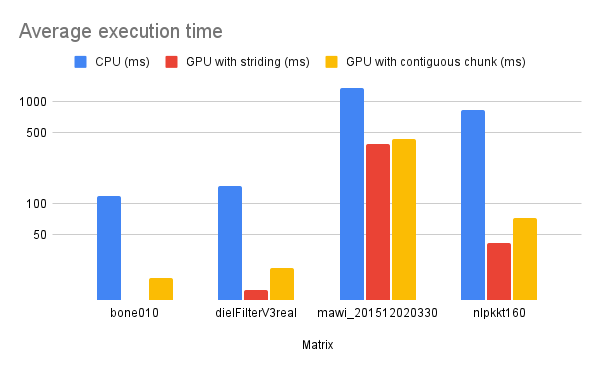
\includegraphics[width=0.95\linewidth]{average-execution-time.png}
    \caption{Average Execution Time (lower is better)}
    \label{fig:avg-exec-time}
\end{figure}

\begin{figure}[h]
    \centering
    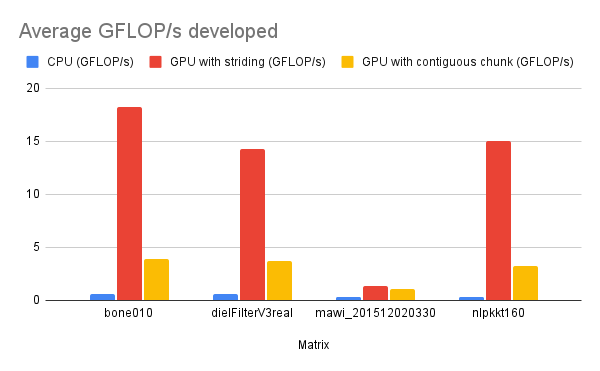
\includegraphics[width=0.95\linewidth]{average-gflop.png}
    \caption{Average GFLOP/s Developed (lower is better)}
    \label{fig:avg-gflop}
\end{figure}
As expected in Section~\ref{sec:methodology} and shown in Figure~[\ref{fig:avg-exec-time},~\ref{fig:avg-gflop}], Algorithm~\ref{alg:striding} is faster than all the other implementations.
\begin{figure}[h]
    \centering
    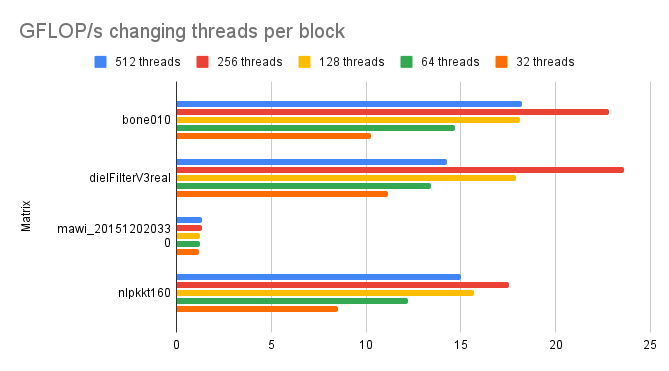
\includegraphics[width=0.95\linewidth]{gflop-block.png}
    \caption{GFLOP Compared The Number Of Threads Per Block}
    \label{fig:gflop-block}
\end{figure}

\begin{figure}[h]
    \centering
    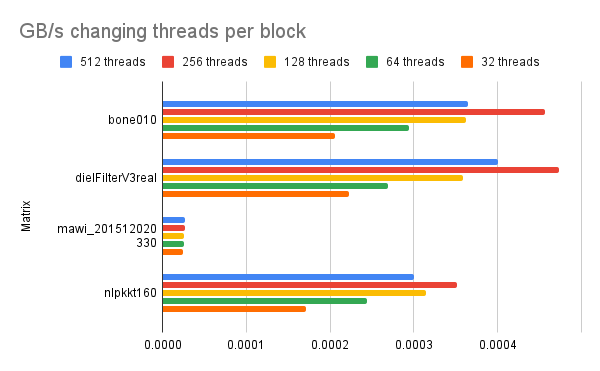
\includegraphics[width=0.95\linewidth]{gb-block.png}
    \caption{GB/s Compared The Number Of Threads Per Block}
    \label{fig:gb-block}
\end{figure}
I decided to dig a bit more into the performances of Algorithm~\ref{alg:striding} by changing the maximum amount of thread per block. Starting from the base of 512 threads I divided by 2 until reaching 32, i.e., the size of warp. The optimal amount of threads per block resulted to be 256. This is due to the use of an atomic instruction within the code, the semantic of the instruction make concurrent write over the same address sequential; in this case if two threads are working on the same row their sum operations will sequentialised since they are trying to write on the same result address. Using less threads,.i.e., each thread works on more elements; conflicts (threads working) on the same row are reduced to a minimum. However, this minimum is not stable, in fact decreasing again the value to 128, 64 or 32 the performances decreases again, this could be symptom of either:
\begin{itemize}
\item too few threads working, so an excessive workload for each of them;
\item too much threads working on the same row, hence an high number of conflicts on the same row.
\end{itemize}
Unfortunately, I was not able to determine a more fine grain optimisation, since the optimal size depends on the input matrix shape. Figure~[\ref{fig:gflop-block},~\ref{fig:gb-block}] highlights the fact that the variations of performances are not constant over all the matrices considered.

\begin{figure}[h]
\centering
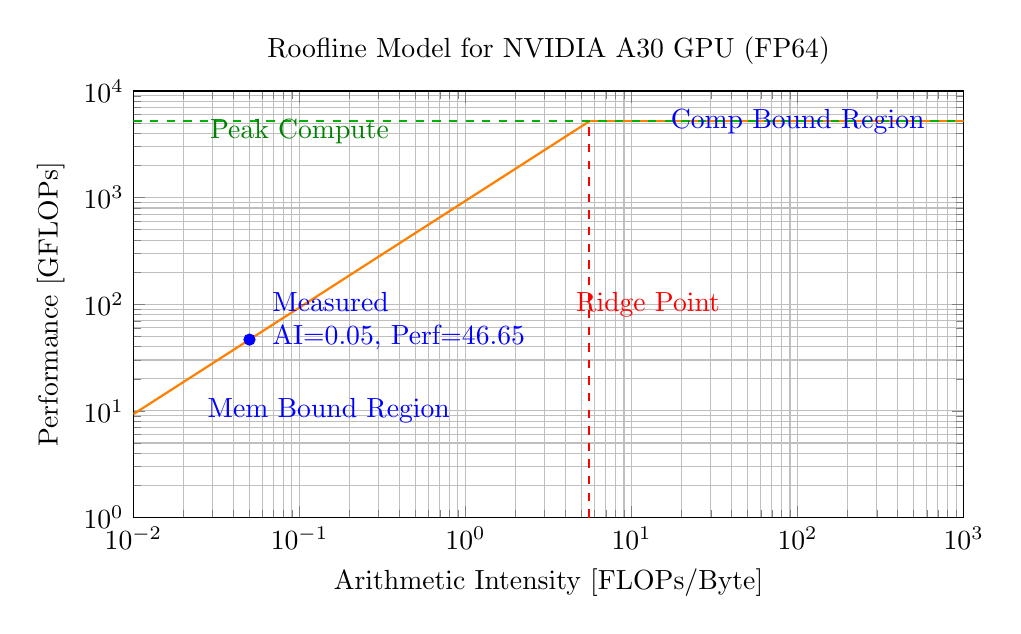
\begin{tikzpicture}
\begin{loglogaxis}[
    width=\linewidth,
    height=7cm,
    xlabel={Arithmetic Intensity [FLOPs/Byte]},
    ylabel={Performance [GFLOPs]},
    title={Roofline Model for NVIDIA A30 GPU (FP64)},
    grid=both,
    xmin=0.01, xmax=1000,
    ymin=1, ymax=10000,
    xtick={0.01, 0.1, 1, 10, 100, 1000},
    ytick={1, 10, 100, 1000, 10000}
]


% --- Parameters ---
\def\ridgepoint{5.57}     % FLOPs/Byte
\def\peakcompute{5200}    % GFLOPs
\def\bandwidth{933}       % GB/s
\def\ArithmeticIntensity{0.05}
\def\performance{46.65}

% --- Roofline: Memory-bound and compute-bound ---
\addplot[
    domain=0.01:\ridgepoint,
    samples=200,
    thick,
    orange
] {\bandwidth * x}; % Memory-bound line

\addplot[
    domain=\ridgepoint:1000,
    samples=2,
    thick,
    orange
] {\peakcompute}; % Compute-bound line

% --- Dashed Ridge point ---
\addplot[dashed, red, thick] coordinates {(\ridgepoint, 1) (\ridgepoint, \peakcompute)};
\node[red] at (axis cs:\ridgepoint + 7, 100) {Ridge Point};

% --- Measured point ---
\addplot[
    only marks,
    mark=*,
    mark size=2pt,
    color=blue
] coordinates {(\ArithmeticIntensity, \performance)};
\node[align=left, anchor=west, blue] at (axis cs:0.06, 70) {Measured\\AI=0.05, Perf=46.65};

% --- Peak compute line (green dashed) ---
\addplot[dashed, green!70!black, thick] coordinates {(0.01, \peakcompute) (1000, \peakcompute)};
\node[anchor=south, green!50!black] at (axis cs:0.1, \peakcompute/2) {Peak Compute};

% --- Annotations ---
\node[blue] at (axis cs:0.15, 10) {Mem Bound Region};
\node[blue] at (axis cs:100, \peakcompute) {Comp Bound Region};

\end{loglogaxis}
\end{tikzpicture}
\caption{Roofline Model For SpMV On NVIDIA A30}
\label{fig:roofline}
\end{figure}

Following the NVIDIA's white-paper for the A30, I drew the roofline model for double precision floating point, since in my code I used \texttt{double} as data type. Figure~\ref{fig:roofline} highlights the fact that my \emph{CUDA} kernels are indeed a memory bounded.

\section{Conclusions}
The presented algorithms are far from decent implementations. The representation used for the matrices is sub-optimal since the length of a row is unknown a priori, therefore it is impossible to do a decent load balancing between the threads. For better GPU performances using another representation such as CSR would works better.

Another bottleneck for the algorithm is represented by the use of an atomic instruction. Instead of this instruction thread/warp level synchronisation should be used.

On the CPU side, this representation is optimal since it permits to maximise the number of cache hits working on data stored so closely.

\bibliographystyle{IEEEtran}
\bibliography{references}

\end{document}

